\section{Métodos superiores}
Os quatro algoritmos classificados como superiores são aqueles que possuem complexidade de tempo de ordem \bigO{n \log n}. Tal complexidade permite a realização de testes com vetores de tamanho consideravelmente maiores do que os utilizados para os algoritmos inferiores, razão pela qual foram testados com vetores cujo tamanho varia de $10^4$ a $10^8$.

\subsection{Tempo de execução}
Foram gerados dois gráficos para apresentar os resultados de tempo de execução. O primeiro, na Figura \ref{fig:superiores1e7-tempo}, mostra os resultados com o tamanho dos vetores limitado a $10^7$, e o segundo, na Figura \ref{fig:superiores1e8-tempo}, apresenta os tamanhos que atingem $10^8$.

\begin{figure}[H]
\Caption{\label{fig:superiores1e7-tempo}Métodos superiores – Tamanho (até $10^7$) × Tempo.}
\centering
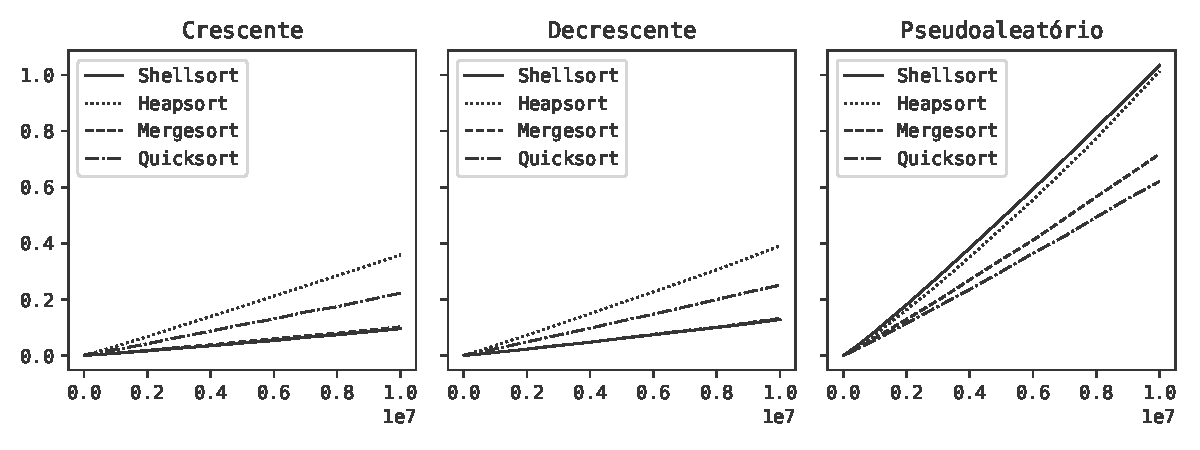
\includegraphics[scale=0.787]{figuras/pdf/superiores1e7.tempo.pdf}
\Fonte{Elaborado pelo autor}
\end{figure}

\begin{figure}[H]
\Caption{\label{fig:superiores1e8-tempo}Métodos superiores – Tamanho (até $10^8$) × Tempo.}
\centering
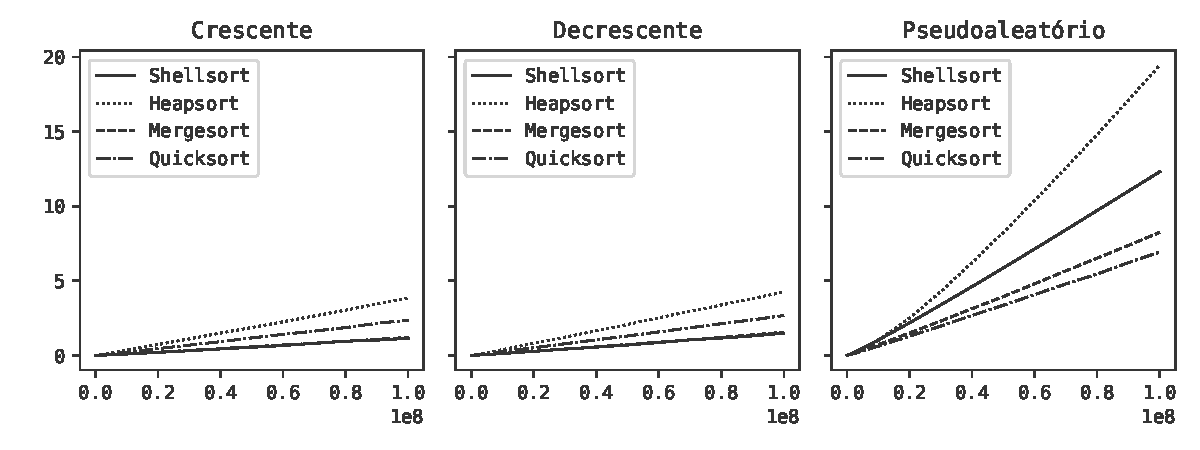
\includegraphics[scale=0.787]{figuras/pdf/superiores1e8.tempo.pdf}
\Fonte{Elaborado pelo autor}
\end{figure}

Para vetores inicialmente ordenados em ordem crescente ou decrescente, não há diferença significativa no comportamento entre a Figura \ref{fig:superiores1e7-tempo} e a Figura \ref{fig:superiores1e8-tempo}. Os algoritmos mantêm a mesma relação de desempenho entre si. Nesses casos, o Heapsort e o Quicksort apresentam seus piores cenários de execução, enquanto o Shellsort e o Mergesort se beneficiam da presença de ordem nos dados.

Já no caso geral, em ambos os gráficos, o Quicksort apresenta o melhor resultado, sendo seguido pelo Mergesort. No entanto, observa-se um comportamento atípico no Heapsort. Para vetores com tamanhos até $10^7$, como esperado pela análise teórica de complexidade, o Heapsort supera o Shellsort. Porém, para tamanhos maiores que $10^7$, o Heapsort se torna ligeiramente mais lento que todos os outros. Este fato será explicado na subseção \ref{subsec:sup-cache}.

\subsection{Comparações}
O gráfico da Figura \ref{fig:superiores.comparacoes} a seguir, exibe a relação entre o número de comparações e o tamanho do vetor para cada tipo de vetor analisado.

\begin{figure}[H]
\Caption{\label{fig:superiores.comparacoes}Métodos superiores – Tamanho × Comparações.}
\centering
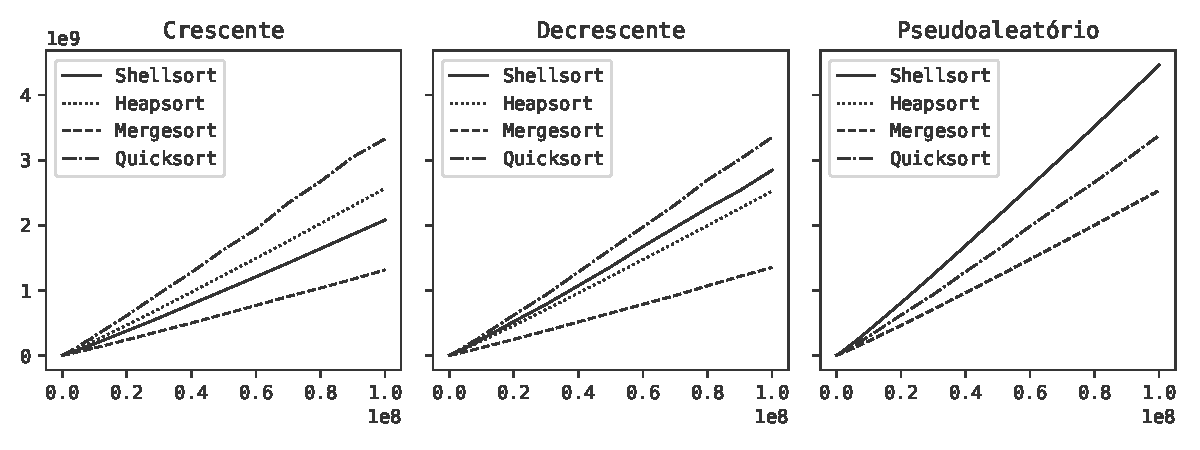
\includegraphics[scale=0.787]{figuras/pdf/superiores.comparacoes.pdf}
\Fonte{Elaborado pelo autor}
\end{figure}

Em contraste com os demais, o Quicksort e o Heapsort demonstraram estabilidade em seu desempenho. Em todos os tipos de vetor, os gráficos de ambos os algoritmos são praticamente idênticos, o que indica que a ordem inicial dos dados não os beneficia nem os prejudica. No entanto, o Heapsort executa um número ligeiramente menor de comparações do que o Quicksort.

Já o Shellsort apresentou um desempenho variável conforme o tipo de vetor. Apesar de se beneficiar quando há presença de ordem nos dados, ele foi, no caso geral, o algoritmo superior que mais executou comparações.

O Mergesort executa o menor número de comparações para todos os três tipos de vetor analisados, destacando-se em vetores já ordenados. Há uma explicação interessante para este fato: o algoritmo Mergesort só executa comparações durante o processo de Merge, e este processo se torna determinístico para vetores ordenados. Esse trecho do algoritmo é mostrado abaixo.

\lstinputlisting[language=C]{codigos/aux/merge_snippet.txt}

\subsection{Movimentações}
O gráfico da Figura \ref{fig:superiores.movimentacoes} a seguir, exibe a relação entre o número de movimentações e o tamanho do vetor para cada tipo de vetor analisado.

\begin{figure}[H]
\Caption{\label{fig:superiores.movimentacoes}Métodos superiores – Tamanho × Movimentações.}
\centering
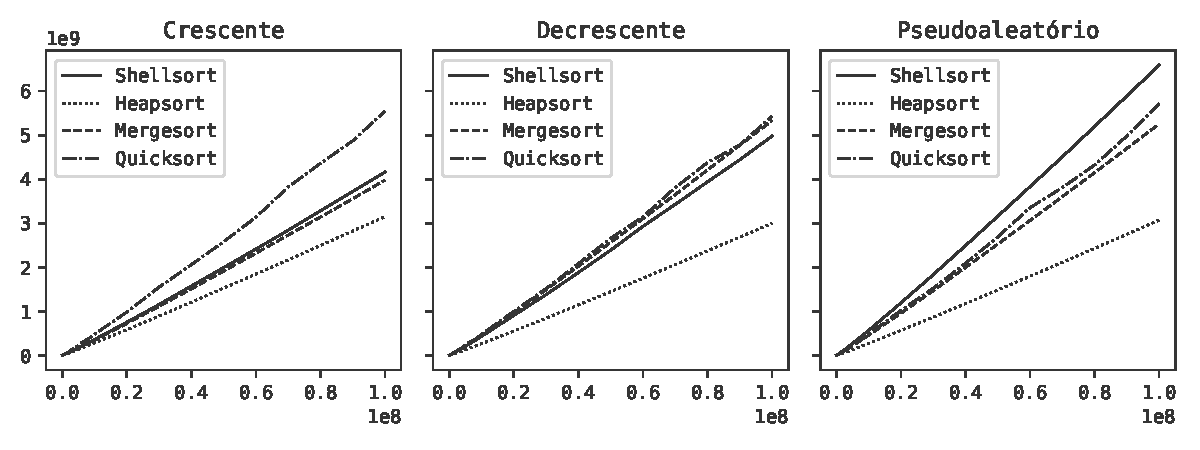
\includegraphics[scale=0.787]{figuras/pdf/superiores.movimentacoes.pdf}
\Fonte{Elaborado pelo autor}
\end{figure}

Com relação à quantidade de movimentações, o algoritmo Heapsort se destacou. Ele manteve o mesmo desempenho em todos os tipos de vetor, mas executou significativamente menos movimentações que os demais algoritmos superiores. O Quicksort também teve desempenho estável para todos os tipos de vetores, sendo ele o que mais executa movimentações para entradas já ordenadas de alguma forma. Já o Mergesort apresentou o mesmo desempenho em vetores decrescentes e no caso geral, mas executou menos movimentações para vetores crescentes, o que ocorre pelo mesmo motivo explicado na subseção anterior. De modo geral, o Shellsort é o que mais realiza a operação de movimentação de elementos do vetor de entrada.

\subsection{Eficiência de cache}\label{subsec:sup-cache}
Conforme introduzido na seção \ref{sec:arquitetura}, o processador tenta realizar a leitura e a escrita primeiramente no cache. Somente quando a informação de interesse não está presente em nenhum nível de cache, é que ele a busca na memória principal. Devido aos tamanhos de vetores utilizados neste trabalho, não é necessário mencionar a memória secundária, uma vez que toda a informação cabe na memória principal. A eficiência de cache de um algoritmo é, portanto, a taxa de sucesso na busca por elementos no cache, visto que esse acesso é muito mais rápido do que na RAM.

\subsubsection{Falhas de leitura}
O gráfico da Figura \ref{fig:superiores-DLmr} mostra a frequência em que o processador falhou ao tentar ler um dado no último nível de cache para cada algoritmo. Observe que, para vetores de tamanhos até $10^7$, e dadas as propriedades do computador utilizado nos testes, praticamente todas as leituras resultavam em sucesso. No entanto, para vetores maiores que isso, as falhas se tornaram visíveis, com o Heapsort sendo o algoritmo que mais apresentou falhas de leitura.

A explicação para a ineficiência do Heapsort reside no princípio da localidade de referência espacial, conforme detalhado na subseção \ref{subsec:localidade-referencia}. Isso ocorre porque, à medida que o algoritmo desce pelos nós do Heap, o índice de cada posição acessada é pelo menos o dobro do índice da posição acessada anteriormente. Essa característica força o carregamento de elementos novos e distantes no cache, os quais se tornam inúteis já na próxima iteração.

\begin{figure}[H]
    \Caption{\label{fig:superiores-DLmr}Métodos superiores – Falhas de leitura no último nível de cache.}
    \centering
    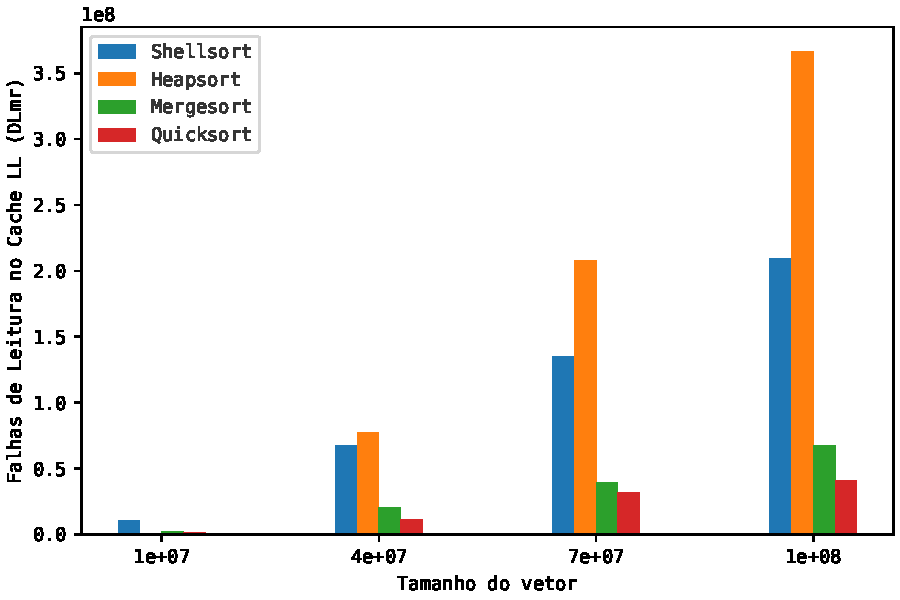
\includegraphics[scale=0.787]{figuras/pdf/superiores_DLmr.pdf}
    \Fonte{Elaborado pelo autor}
\end{figure}

\subsubsection{Falhas de escrita}
O gráfico da Figura \ref{fig:superiores-DLmw} mostra a frequência em que o processador falhou ao tentar escrever um dado no último nível de cache para cada algoritmo. Percebe-se que, mais uma vez, a quantidade de falhas é insignificante para vetores menores que $10^7$. Constata-se também que apenas o Mergesort causa falhas desse tipo. Este fato é explicado pela necessidade deste algoritmo de usar memória auxiliar.

\begin{figure}[H]
\Caption{\label{fig:superiores-DLmw}Métodos superiores – Falhas de escrita no último nível de cache.}
\centering
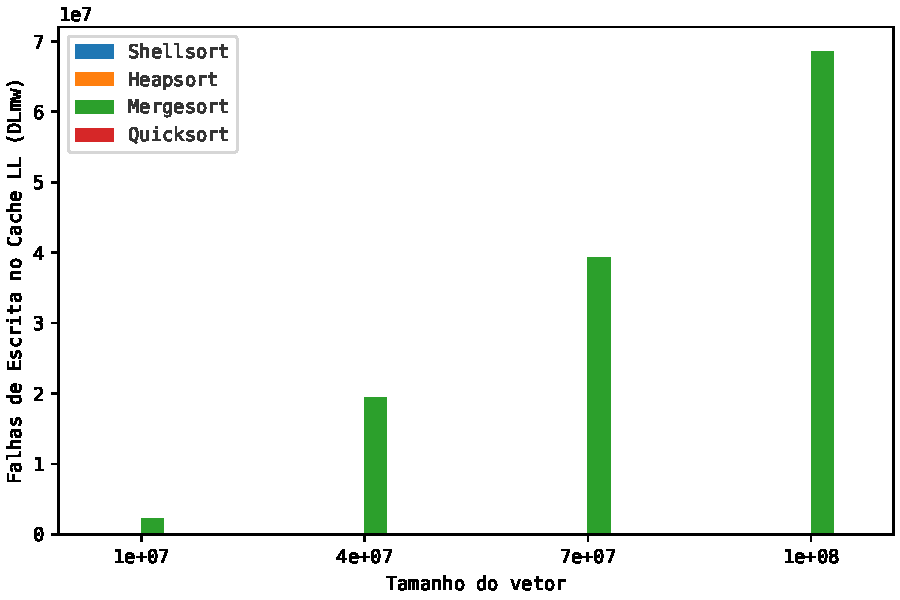
\includegraphics[scale=0.787]{figuras/pdf/superiores_DLmw.pdf}
\Fonte{Elaborado pelo autor}
\end{figure}

\subsection{Síntese dos resultados}
A Table \ref{tab:sup-classicacao} a seguir classifica os algoritmos superiores por tempo, comparações, movimentações e uso do cache, no caso geral.

\begin{table}[H]
    \centering
    \Caption{\label{tab:sup-classicacao}Métodos superiores – Classificação de desempenho por métrica}
    \begin{tabular}{ | c | l | l | l | l | l | }
        \hline
        Ranking & Tempo     & Comp.     & Movi.     & Leitura   & Escrita   \\
        \hline
        1º      & Quicksort & Mergesort & Heapsort  & Quicksort & Shellsort \\
        2º      & Mergesort & Heapsort  & Mergesort & Mergesort & Heapsort  \\
        3º      & Shellsort & Quicksort & Quicksort & Shellsort & Quicksort \\
        4º      & Heapsort  & Shellsort & Shellsort & Heapsort  & Mergesort \\
        \hline
    \end{tabular}
\end{table}

O Quicksort, apesar de não ser o algoritmo que realiza menos comparações ou movimentações, é o mais eficiente em termos de cache. Essa eficiência o estabelece como o melhor algoritmo superior para a principal métrica, o tempo. Já o Shellsort é o que mais executa comparações e movimentações, mas ainda assim acaba sendo mais rápido que o Heapsort, também devido à sua eficiência de cache. Por fim, o Mergesort é quase tão bom quanto o Quicksort, sendo penalizado pelo uso de memória extra.
